\documentclass[a4paper, titlepage, oneside]{article}

\usepackage[utf8]{inputenc}
\usepackage[australian]{babel}
\usepackage[vmargin = 2 cm, hmargin = 2 cm]{geometry}
\usepackage{multicol}
\usepackage{csquotes}
\usepackage{amsmath, amssymb}
\usepackage[cdot, amssymb]{SIunits}
\usepackage{graphicx, float}
\usepackage[outdir = ./build/]{epstopdf}
\usepackage{aasmacros}
\usepackage[backend = biber, style = authoryear, alldates = iso8601]{biblatex}
\usepackage[colorlinks = true, pdfpagemode = UseNone, pdfstartview = FitH]{hyperref}
\usepackage{setspace}

% \usepackage{listings}
% \usepackage{xcolor}
% \usepackage{csvsimple}

% inputenc  : UTF-8 support for non-ASCII characters
% babel     : set language, for packages that need it
% geometry  : page margins
% multicol  : multiple columns
% csquotes  : context-sensitive quotes
% amsmath   : maths
% amssymb   : maths (\square redefined by SIunits)
% SIunits   : management of SI units; encourage using \unit{value}{units} command whenever possible
% graphicx  : \includegraphic
% float     : float graphics
% epstopdf  : use of eps files in document
% aasmacros : CUSTOM - assumes user has aasmacros.sty installed
% biblatex  : bibliography
% hyperref  : in-document links

% listings  : import external code
% xcolor    : more powerful engine for colour formatting
% csvsimple : import csv tables

% biblatex setup
\renewcommand{\nameyeardelim}{\addcomma\addspace} % Change delimiter for in-line citations to include a comma
\addbibresource{group-report.bib}

% hyperref setup
% \hypersetup{allcolors = blue} % Override all link colours
% \hypersetup{hidelinks} % Links will be shown with neither boxes nor colours

% table setup
\renewcommand{\arraystretch}{1.2} % table row spacing increases!

% Custom macros
\newcommand{\elem}[2]{\textsuperscript{#1}{#2}}
\newcommand{\molec}[2]{\ensuremath{\text{#1}_{#2}}}
\newcommand{\ion}[2]{#1~\smallcaps{#2}} % Must use lowercase Roman numerals eg, \ion{H}{ii}
\newcommand{\e}[1]{\ensuremath{\times 10^{#1}}}
\newcommand{\smass}{\mathrm{M_\odot}}
\newcommand{\parsec}{\mathrm{pc}}
\newcommand{\erg}{\mathrm{erg}}
\newcommand{\photon}{\mathrm{ph}}

% Document
\begin{document}
\title{\textbf{Searching for molecular gas towards TeV gamma-ray sources: Analysing 3D data cubes of the molecular gas tracer carbon monoxide with images from the HESS gamma-ray telescopes}}
\author{R.~M. Harvey \and K.~T. Leaver \and H.~D. Poulter}
\date{13 October 2014} %Leave blank to print no date, or you can type in the desired date
\begin{titlepage}
\begin{center}
~

\vfill

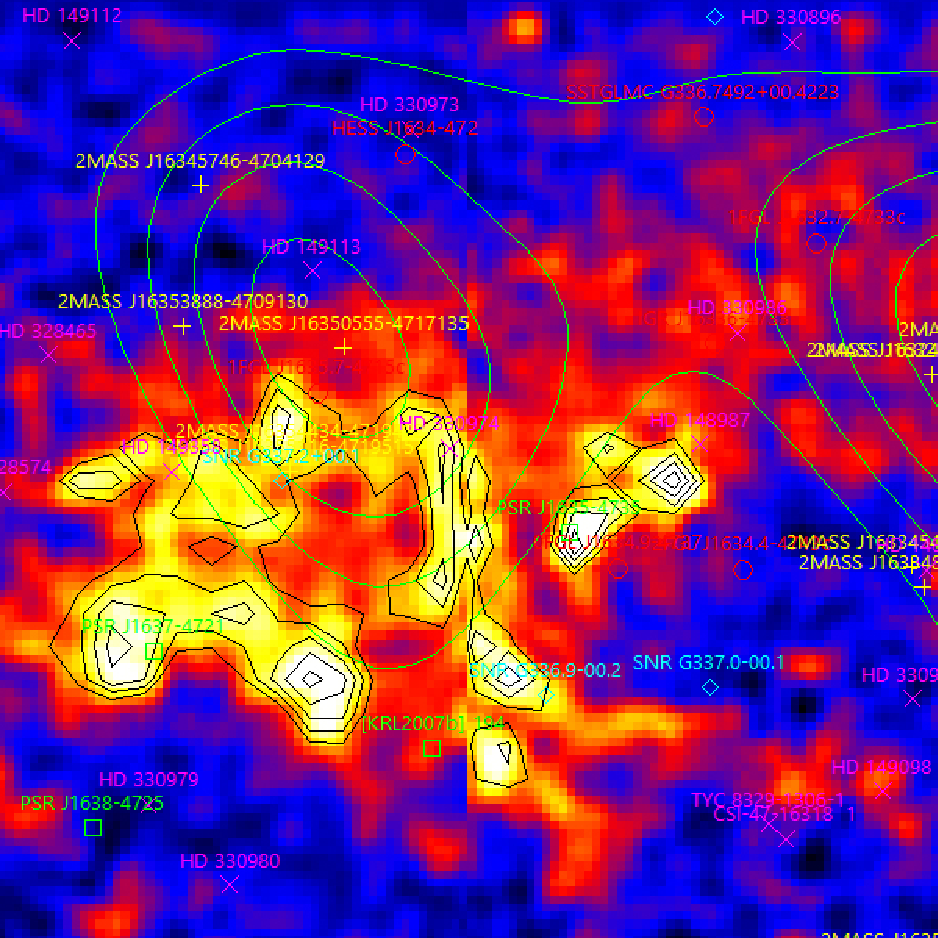
\includegraphics[width = 0.7\textwidth]{figures/cover-pic}

\vspace{1em}

\begin{spacing}{1.9}
{\LARGE \textbf{Searching for molecular gas towards TeV gamma-ray sources: Analysing 3D data cubes of the molecular gas tracer carbon monoxide with images from the HESS gamma-ray telescopes}}

\vspace{2.5em}

{\large R.~M. Harvey \quad\quad\quad K.~T. Leaver \quad\quad\quad H.~D. Poulter}
\end{spacing}

\vspace{1em}

{\large \today}

\vfill

~

\end{center}
\end{titlepage}

\setcounter{page}{1}
\pagenumbering{roman}
\numberwithin{equation}{section}

\tableofcontents

\clearpage
\setcounter{page}{1}
\pagenumbering{arabic}

\begin{center}
  {\large \textbf{Searching for molecular gas towards TeV gamma-ray sources: Analysing 3D data cubes of the molecular gas tracer carbon monoxide with images from the HESS gamma-ray telescopes}}

  \vspace{1.5em}

  R.~M. Harvey\footnote{Molecular clouds, Kinematics, HESS J1634-472} \quad K.~T. Leaver\footnote{Featured telescopes, Carbon monoxide as a tracer for molecular hydrogen, HESS J1640-465} \quad H.~D. Poulter\footnote{Cosmic ray sources, Galactic rotation, Noise anaylsis, Carbon monoxide clouds, HESS J1632-479}
\end{center}

\vspace{1.5em}

\begin{minipage}{0.93\textwidth}
  \begin{abstract} % finish properly
  This report is about finding possible source candidates for HESS J1632-479, HESS J1634-472 and HESS J1640-465 through studying molecular clouds towards these sources. It beings with a brief overview of the types of physical and astronomical concepts behind the science that has been used in writing up the report, before describing the methods used in analysing the data, and then presenting the findings of the data analysis with regards to source candidates for each gamma-ray source. The report found that some sources in HESS J1632-479 and HESS J1640-465 were energetic enough to be linked to the large gamma-ray output
  \end{abstract}
\end{minipage}

\vspace{1em}

\begin{multicols}{2}
\section{Introduction}
\paragraph{}
TeV gamma-ray sources are among the most energetic sources known to exist in the universe. They are theorised to originate from cosmic ray sources, which are some of the more exotic astrophysical objects. This report aims to cover the theory behind searching for possible explanations behind these powerful sources, as well as give insight into analytical techniques used in processing the data, leading to a final consideration of possible causes of these gamma-ray sources.

\section{Theory}
\paragraph{}
This report deals with many different astrophysical concepts in its analysis and such. In order to gain a more complete understanding of the work being done, this section aims to outline them. Due to the large array of different energy schemes present in analysing TeV gamma-rays, data from different telescopes and observatories were used in producing an analysis of the results. Data from different energy regimes was required due to the large collection of possible cosmic ray sources that could result in gamma-ray emission at the TeV scale. Data from Mopra is given special treatment due to its ability to map CO distributions in three dimensions -- this effect arising from galactic rotation. Arguably more importantly however, are the mechanisms behind the different regimes of cosmic ray interactions, mostly with giant molecular clouds. A discussion of CO as a tracer for such molecular clouds is also given.

\subsection{Featured telescopes}
\paragraph{} \label{sec:tel}
The HESS Cherenkov Telescope system is a telescope array that detects high energy gamma rays (\(\sim\)\(3\e{10}\) to \unit{10^{14}}{\electronvolt}). We received data showing the detected intensity for the three gamma ray sources as single frame fits files, the value associated with each pixel representing the number of gamma ray counts in the energy band of the observations. This data allowed the location, intensity and extent of the three sources to be determined. The primary data used to analyse the potential source candidates for the gamma rays was gathered by the Mopra Radio Telescope. Data for both \elem{13}{C}O and \elem{12}{C}O (see section~\ref{sec:co}) was used in data cube format, where the doppler shift of the emission lines of the CO has been convcerted to relative velocity. The data cube contains several thousand frames that span \(\sim\)\unit{1000}{\kilo\meter\cdot\reciprocal\second} and are used to represent the distance to the source of the emissions.

\subsection{Cosmic ray sources}
\paragraph{} \label{sec:cr}
Cosmic rays are highly-relativistic charged particles with very large associated energies in the order of GeV--TeV. They originate from some of the most extreme environments in the universe, and understanding this is essential in studying the sources of such particles. Cosmic rays sources act as particle accelerators, with large electric and magnetic fields accelerating charged particles to the high energies seen in space. Sources include supermassive blackholes at galactic centres, such as the one at the centre of the Milky Way \parencite{Guo:2013}, massive star clusters, supernova remnants \parencite{Vink:2013} and pulsars -- typically those that have been newly-formed and are capable of accelerating charged particles to extreme energies \parencite{Fang:2012}.

Due to cosmic rays being charged in nature, their path through space will not be in a straight line like that of light. Instead, due to magnetic fields, it will change directions so when such particles are detected on Earth by air shower, their direction will not be an accurate representation of the location of the source from where they originated from \parencite{Kalli:2011}. Rather than looking directly for cosmic rays in order to find their sources, it makes more sense to look for the effect cosmic rays have on their surrounds, and draw conclusions as to their origins from those. As an example, supernova remnants (SNRs) that are capable of producing cosmic rays may also produce gamma rays as a consequence of the cosmic ray interaction with the nebula.

\subsection{Galactic rotation}
\label{sec:gal-rot}
\paragraph{}
The Mopra data featured heavily in this report \parencite{Burton:2013} derives its usefulness from the effect that galactic rotation has on objects along the line of sight across the Milky Way. Fig.~\ref{fig:gal-rot} shows how for a simplified model of the Milky Way with constant radial velocity, looking along a line of sight, in this particular instance one corresponding to a galactic latitude of \(l=337\), leads to a velocity gradient and a measurable Doppler shift. In order to find distances from the sun using the Mopra data, it is necessary to consider the component of velocity parallel to the line of sight. It is also worth noting that the Mopra data measures velocity with respect to the local standard of rest (LSR). As derived in Appendix~\ref{app:doppler}, the velocity of an object along the line of sight with galactic latitude \(l\) is given by
\begin{equation}
  v_{los}(d)=\frac{v(R)R_0\sin{l}}{\sqrt{d^2-2R_0d\cos{l}+R_0^2}}-v(R_0)\sin{l}\;\,,
\end{equation}
where the distance from the LSR to the galactic centre (GC) is \(R_0\), and distance from the LSR to the object of interest is \(d\). This equation holds for a galaxy with variable rotation \(v(R)\) dependent on radial distance \(R\) from the GC. For the sake of simplicity in this report, this expression is taken to be a constant \(v(R)=\unit{255.2}{\kilo\metre\usk\reciprocal\second}\), as suggested by recent very-long-baseline interferometry carried out by \textcite{Reid:2014}. They also suggest a value for the distance from the GC to be \(R_0=\unit{8.36}{\kilo\parsec}\).

\begin{figure}[H]
  \centering
  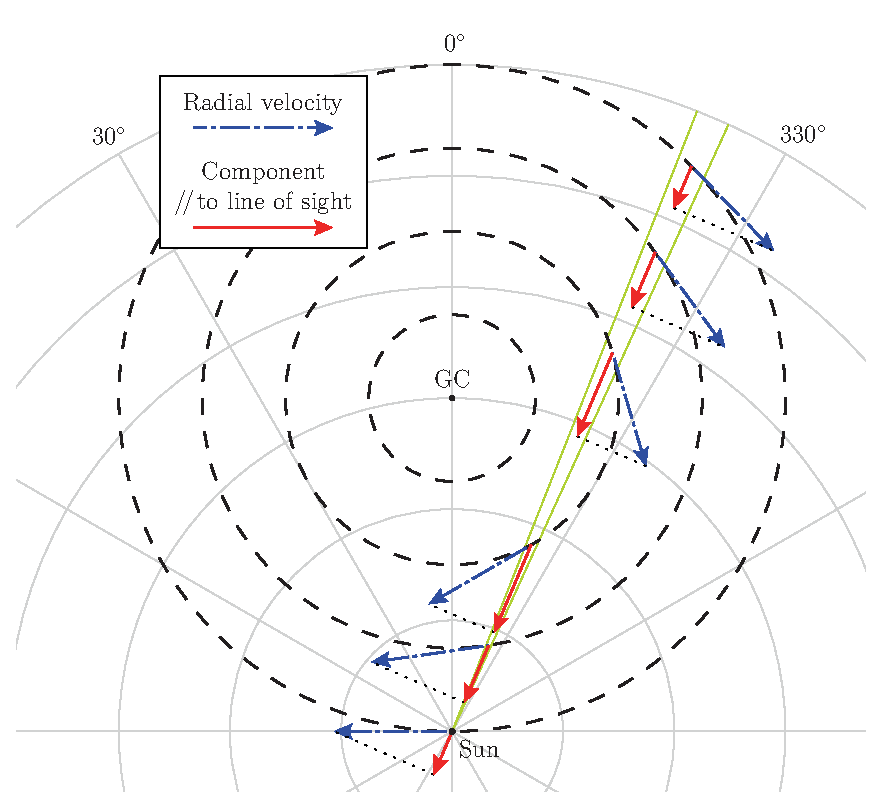
\includegraphics[width = \columnwidth]{figures/galactic-rotation}
  \caption{Galactic rotation showing Doppler shifts}
  \label{fig:gal-rot}
\end{figure}

\subsection{Molecular clouds}
\subsubsection{Composition and structure}
\paragraph{}
The average density of the interstellar medium (ISM) is quite low, however the reaches of space are littered with so-called molecular clouds -- areas with gas and dust density significantly higher, such that stars can form within the material. These clouds are predominantly composed of molecular hydrogen (\molec{H}{2}), which for reasons to be discussed in Section~\ref{sec:co} is relatively difficult to detect. However, the presence of carbon monoxide (CO) is significantly easier to determine, and astrophysicists presently believe it to be distributed among \molec{H}{2} in effectively equal quantities, making it an excellent tracer \parencite{Glover:2011}.

Gas and dust formations with a total mass between \(10^3\) and \unit{10^7}{\smass} are called giant molecular clouds (GMCs), and tend to be anywhere from 5 to 200 parsecs in diameter \parencite{Murray:2011}. `Diameter' is a term applied fairly loosely, as the form of a GMC is not guaranteed to be even remotely spherical. Indeed, the tenuous structural qualities of GMCs mean that they can also vary greatly in density, typically from around \(2\e{-20}\) to \unit{2\e{-18}}{\gram\usk\centi\metre\rpcubed}, corresponding to approximately \(10^4\) to \(10^6\) molecules per cubic centimetre \parencite{Ferriere:2001}.

\subsubsection{Interactions with cosmic rays}
\paragraph{}
Cosmic rays incident on GMCs can through a variety of mechanisms produce gamma rays, in our case often within TeV range and hence detectable by the HESS telescope. Bremsstrahlung radiation is motivated by Coulombic forces, and results from inbound cosmic rays being deflected by charged particles present in the interstellar gas, this change thus emitting gamma radiation. Inverse Compton scattering is motivated by conservation of momentum, and involves high-energy cosmic rays colliding with ``soft'' photons in the gas, exchanging momentum and in the process resulting in a more energetic photon with energies in TeV ranges \parencite{Ferriere:2001}. The synchrotron effect may also produce gamma rays, but is not included in this data set as HESS is not sensitive to such effects.

\subsubsection{Kinetic energy of expanding bubbles}
\label{sec:kinetic}
\paragraph{}
Powerful events in GMCs -- such as supernovae -- can push away all nearby gas, clearing out distinct ``bubble'' regions readily visible in images of gas distributions. In order to find the energy released by the event, we simply need find the kinetic energy of the gas which is now moving away, assuming it previously had negligible kinetic motion and almost all of the energy released by the event has been transferred to the surrounding gas.

The Mopra data cubes provide redshift speeds for each image slice, hence permitting us to find the relative speeds of two areas of gas, such as the two sides of an expanding bubble. For the full derivation please see Appendix~\ref{app:kinetic}, however the final result is replicated here:
\begin{equation}
  \label{eq:KE}
  \mathrm{KE} = \frac{\pi ^ 4}{6} {\left( \frac{\Delta l}{360} \right)}^3 \rho d^3 {(v_1 - v_2)}^2 \, \joule \, ,
\end{equation}
where \(\Delta l\) is the maximum angular width of the bubble in degrees, \(\rho\) is an estimate of the mass density in \(\kilo\gram\usk\centi\metre\rpcubed\) of the gas previously occupying that volume, \(d\) is the distance to the centre of the bubble in \(\centi\metre\), and \(v_1\) and \(v_2\) are the redshift speeds of the front and back of the bubble in \(\metre\usk\reciprocal\second\).

\subsection{Carbon monoxide as a tracer for molecular hydrogen}
\label{sec:co}
\paragraph{}
The majority of the hydrogen in the galaxy is in either atomic or molecular form. Atomic hydrogen can emit a photon because of the energy difference between the electron and proton having parallel and anti-parallel spins. This spin transition for the electron results in the emission of a photon with a wavelength of \unit{21}{\centi\metre}. Molecular hydrogen (\molec{H}{2}) has very weak emission lines due to its high symmetry, and at the extremely low molecular cloud temperatures of \(\sim\)\unit{10}{\kelvin}, molecular hydrogen is completely undetectable. Thankfully, carbon monoxide (CO) is asymmetric and occurs alongside \molec{H}{2} in a mostly uniform ratio throughout our galaxy \parencite{Neininger:1998}. The CO is hit by neighbouring molecules and gains energy in either rotational or vibrational stretching forms. These energy modes are quantised, and when the rotation or vibration drops an energy level a photon will be emitted. Because each isotopologue will have a different moment of inertia and therefore different energy levels, the frequency of the photon will depend on both the isotopologue and the energy levels between which the transition occurs. Because of this it is possible to look for specific isotopologues and specific energy transitions, which, knowing how they are distributed with \molec{H}{2}, allows the mapping of molecular clouds.

\section{Data analysis} % finish properly ? add more maybe
\paragraph{}
In this section, analytical techniques such as noise analysis, kinematic analysis and analysis of the Mopra CO data are outlined and discussed.

\subsection{Noise analysis}
\paragraph{}
A vital aspect of the analysis of data from HESS, Mopra, and other data sources involved estimating the level of background noise associated with each data set, and making judgements regarding the cut-off level where the data became valid signal. Before noise analysis was done proper, it was made sure that for each data set, a Gaussian smoothing of three pixels was applied in order to smooth over any random noise effects present in the data.

Fig.~\ref{fig:noise} shows a schematic idealisation of the histograms for the data sets used in the report. In order to plot accurate contours of gas clouds, and hence properly analyse them, the levels had to be set so that background counts were effectively removed. Each data set has already had a defined number of background counts subtracted from it, thus leading to the existence of points with negative numbers of counts. This in turn meant the formation of an associated background count roughly distributed as a Gaussian curve due to its random nature, as seen in Fig.~\ref{fig:noise}. In order to only plot contours on values considered to be signal, and correctly ignore the background noise, we considered the standard deviation \(\sigma\) of the background. As we expected the number of counts for the signal to be in the positive domain, we focused on the negative side of the histogram and used it to estimate the value of the standard deviation \(\sigma\) in the background noise, using the approximate ``bell curve'' present in the negative domain. In order to be more certain that only the signal was then considered, the value for \(\sigma\) was doubled, and this used as the lower contour limit. Thus, for the normally-distributed background noise, only 2.3\% of the noise would be included in the statistically-significant contour levels. This allowed further analyses on the sources to clearly identify the signal from the noise, and hence have much stronger accuracy.

\begin{figure}[H]
  \centering
  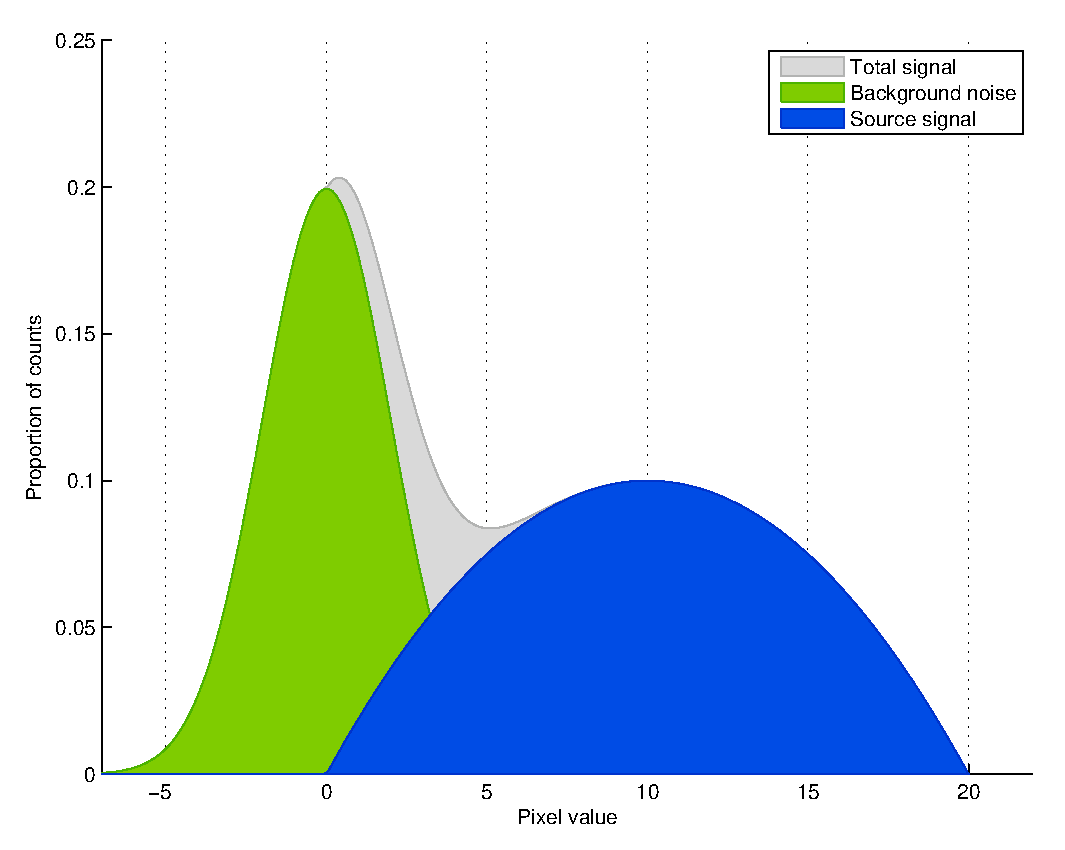
\includegraphics[width = \columnwidth]{figures/noise-analysis}
  \caption{Representative graph of the signal histogram}
  \label{fig:noise}
\end{figure}

\subsection{Kinematics}
\paragraph{}
Several gas clouds have formations highly suggestive of bubbles formed due to supernova explosions. Using the techniques outlined in Section~\ref{sec:kinetic}, we subsequently calculate the energies of those bubbles.

\subsubsection{IGR J16358-4726}

\begin{figure}[H]
  \centering
  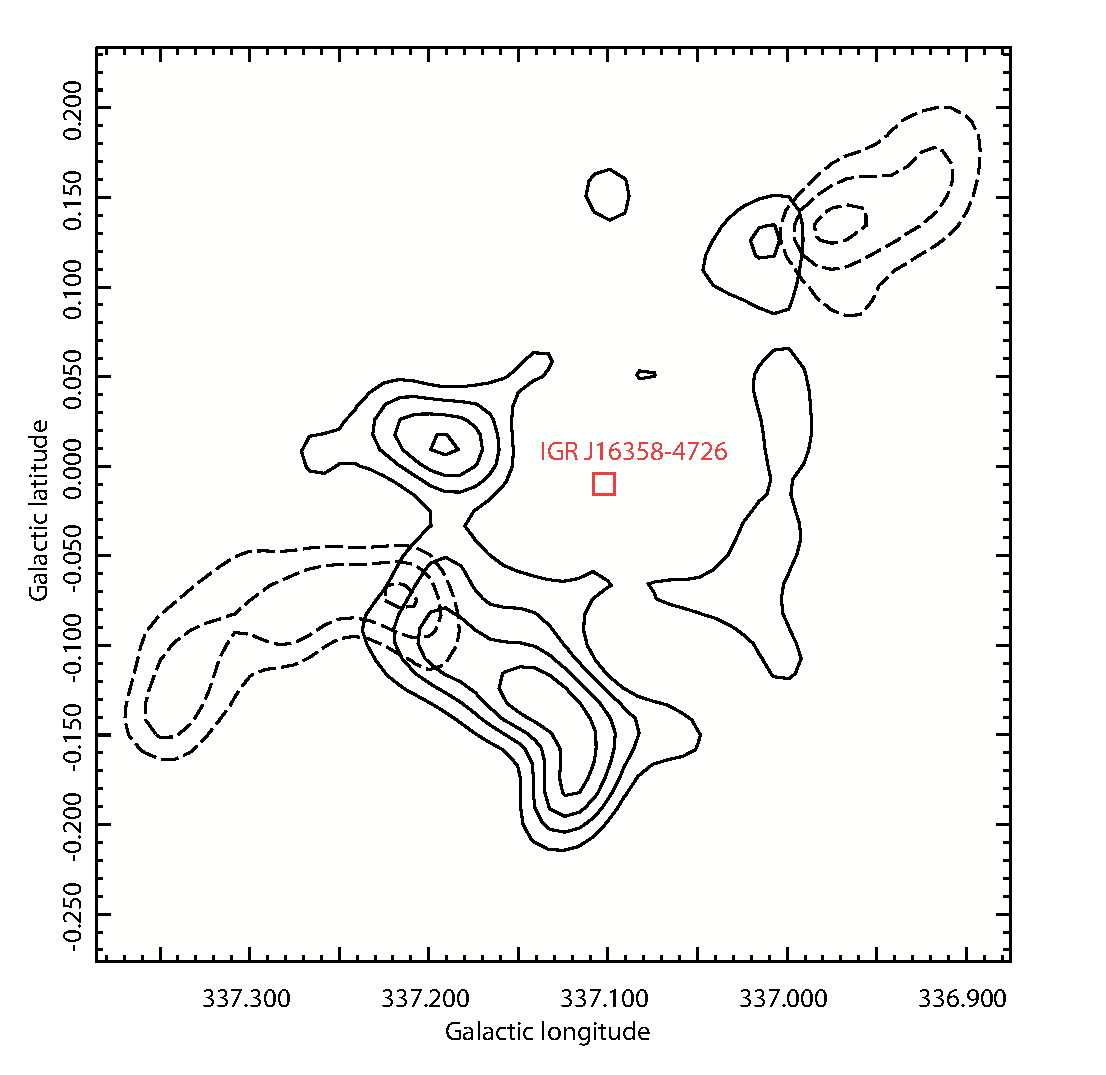
\includegraphics[width = \columnwidth]{figures/bubble34}
  \caption{\elem{13}{C}O composite image of three frames best illustrating the bubble around IGR J16358-4726. The dashed contours are jets, behind (lower left) and in front of (upper right) the central contours of the midsection}
  \label{fig:bubble34}
\end{figure}

\paragraph{}
Fig.~\ref{fig:bubble34} shows the formation of a bubble around IGR J16358-4726, discussed further in Section~\ref{sec:hess34}. Applying Eq.~\ref{eq:d} for \(v(R) = v(R_0) = \unit{255.2\e{3}}{\metre\usk\reciprocal\second}\) and \(R_0 = \unit{8.34}{\kilo\parsec}\) \parencite{Reid:2014}, we find the central object to be either \(4.18\) or \unit{11.2}{\kilo\parsec} away, which agrees quite favourably with \textcite{Lutovinov:2005} who report near and far solutions for distance equal to \(5 - 6\) and \unit{12 - 13}{\kilo\parsec}, respectively. With these distances, we use Eq.~\ref{eq:KE} and assume an average uniform mass density \(\rho\) of \unit{2\e{-21 \mathrm{~to~} -23}}{\kilo\gram\usk\centi\metre\rpcubed} \parencite{Ferriere:2001} to find the bubble has kinetic energy \unit{9.34\e{42 \mathrm{~to~} 44}}{\joule} for the near solution and \unit{1.78\e{44 \mathrm{~to~} 46}}{\joule} for the far solution. Considering the average energy output of a supernova is of the order of \unit{10^{44}}{\joule} \parencite{Khokhlov:1993}, this is a very reasonable result.

\subsubsection{SNR G338.5+00.1}

\begin{figure}[H]
  \centering
  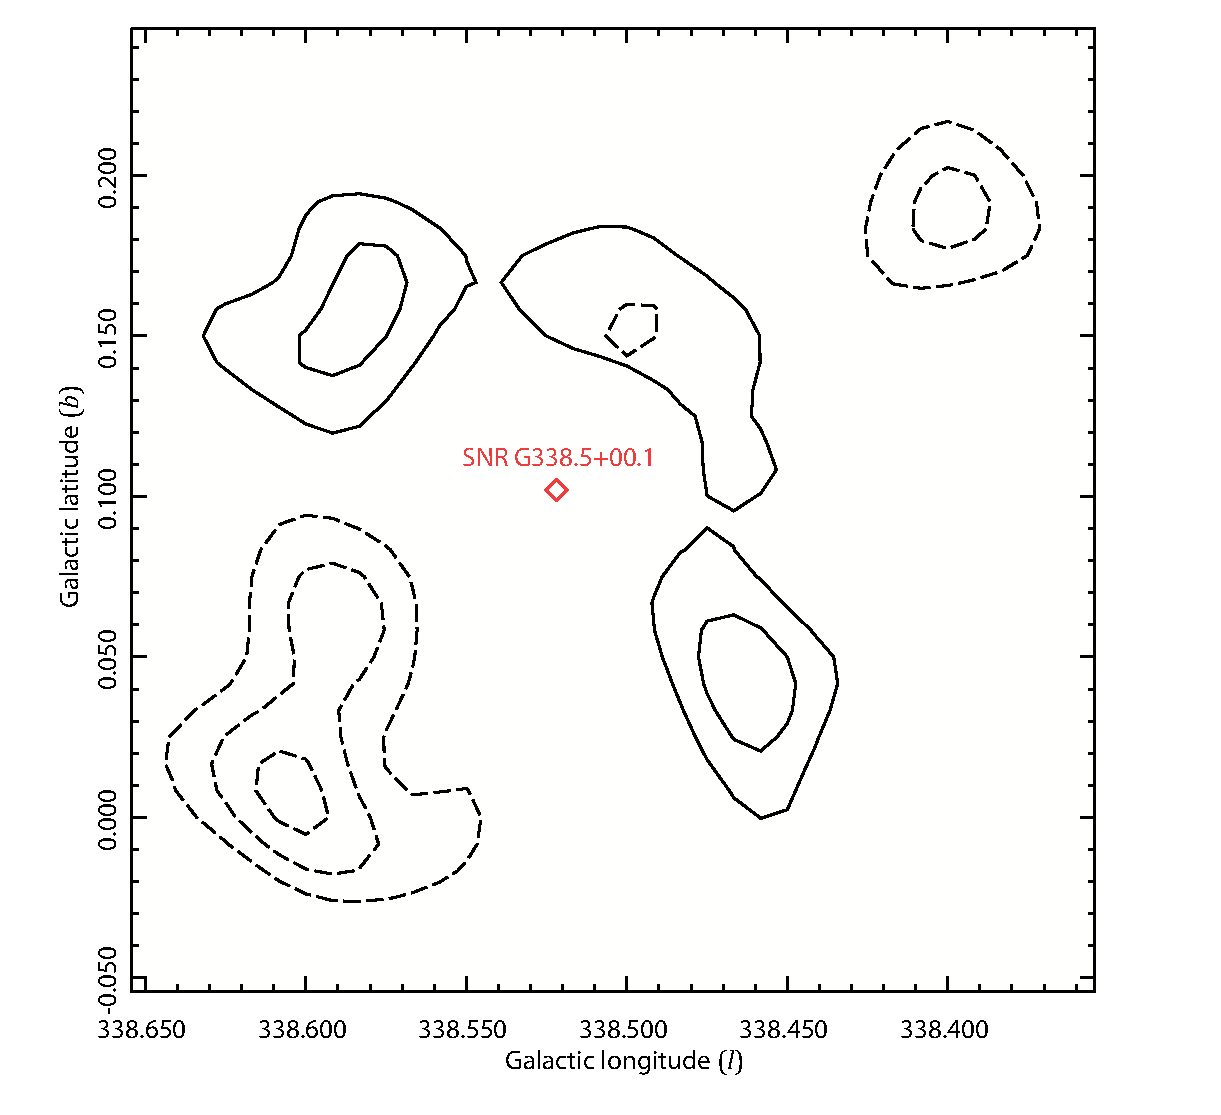
\includegraphics[width = \columnwidth]{figures/bubble40}
  \caption{\elem{13}{C}O composite image of three frames best illustrating the bubble around SNR G338.5+00.1. The dashed contours are jets, behind (lower left) and in front of (upper right) the central contours of the midsection}
  \label{fig:bubble40}
\end{figure}

\paragraph{}
Fig.~\ref{fig:bubble40} shows the formation of a bubble around SNR G338.5+00.1, nearby to HESS J1640-465. We find the object to be either \(2.11\) or \unit{13.4}{\kilo\parsec} away. The near solution is probably \textit{too} near, and the far solution compares well with the sole value of \(\sim\)\unit{11}{\kilo\parsec} given by \textcite{Kothes:2007}. \textcite{Pavlovic:2013} report a single distance of \unit{7.3}{\kilo\parsec}, however they note that their radical new method may have errors of up to 50\%. For the same range of average uniform mass densities as before, we determine kinetic energies of \unit{1.35\e{41 \mathrm{~to~} 43}}{\joule} for the near solution and \unit{3.48\e{43 \mathrm{~to~} 45}}{\joule} for the far solution. Compared to the average energy output of a supernova, these results support the far solution being the sole possible solution, and place it in an ideal energy range.

\subsection{Carbon monoxide clouds}
\paragraph{}
The \elem{12}{C}O and \elem{13}{C}O data cubes from Mopra were analysed slice-by-slice, with any interesting regions of gas recorded in Table~\ref{tab:mopra-obs}. The general approach to analysing the molecular gas clouds was to check for any potential line-up with the HESS gamma ray sources, as well as any bubble structures or other line-up with high energy sources. The high-energy sources considered during analysis were pulsars, supernova remnants, Wolf-Rayet stars, and O, B and A stars, with masers serving as good pointers for star-forming regions.

As well as data from HESS, the Mopra data cubes were also compared against contours from ROSAT and Spitzer to explore the soft x-ray and infrared regime as well for possible indicators as to what regions the CO clouds could correspond to. Any line-up with Spitzer would imply a dense star-forming region, but no line-up was found for ROSAT data.

\section{Source candidates} % finish properly
\paragraph{}
During the analysis of CO data from Mopra, as well as using the SIMBAD catalogue to plot high-energy sources, a few were set aside as possible candidates for the large gamma ray readings from HESS. In this section, the sources are discussed alongside their possible effect on the gamma-ray emission measured from HESS.

\subsection{HESS J1632-479}

\begin{figure}[H]
  \centering
  \frame{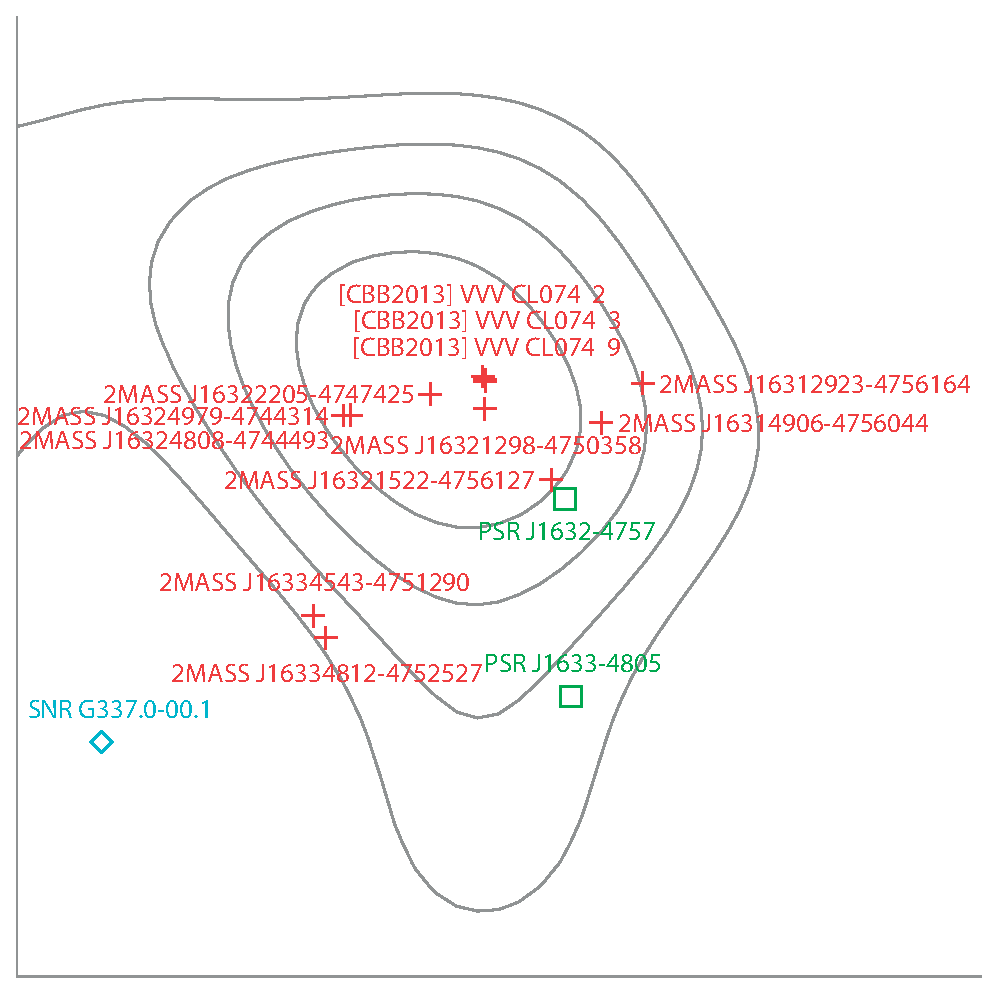
\includegraphics[width = \columnwidth]{figures/hess32}}
  \caption{Contour plot of HESS J1632-479 and surrounding objects of interest. Wolf-Rayet stars are shown as red crosses, supernova remnants as blue diamonds, and pulsars as green squares}
  \label{fig:hess32}
\end{figure}

\paragraph{}
HESS J1634-479 has a photon flux of \unit{28.7\pm5.3\e{-12}}{\photon\usk\centi\metre\rpsquared\usk\reciprocal\second} for energies over \unit{200}{\giga\electronvolt} \parencite{Aharonian:2006}. The source candidates for this particular gamma-ray source include a gamma ray source, 2FGL J1632.4-4753c, a Wolf-Rayet cluster, VVV CL074, as well as a high-mass x-ray binary, IGR J16320-4751.

\subsubsection{2FGL J1632.4-4753c}
\paragraph{}
The most likely candidate for this source would be 2FGL J1632.4-4753c, which is a gamma ray source found by \textcite{Lande:2012}. It is the most energetic of the possible candidates, with an integral flux of \unit{1.4\e{-9}}{\photon\usk\centi\metre\rpsquared\usk\reciprocal\second} \parencite{Lande:2012}. As the distance to this source is unknown, the intrinsic flux associated with it cannot be found, yet it suffices to know that this figure is for photons with energy \(>\unit{10}{\giga\electronvolt}\) meaning it is a very energetic source. \textcite{Lande:2012} also cites the counterpart for this source to be HESS J1632-479, suggesting a strong link between the two sources.

\subsubsection{VVV CL074}
\paragraph{}
An object worthy of attention within this source is VVV CL074, a Wolf-Rayet open star cluster discovered by \textcite{Chene:2013}, which could be contributing to the total gamma ray emission. Worth noting is that in this open cluster one star in particular, VVV CL074 9, is given by \textcite{Chene:2013} to be at a distance of \unit{13.57}{\kilo\parsec}, while other stars in the cluster are within a distance of \unit{8}{\kilo\parsec}. This star in particular has a spectral class of WN7/O4–6If+ \parencite{Chene:2013}, giving it the possibility of it being either a Wolf-Rayet star (WR*) with prominent nitrogen lines in its spectra, or an O-type star with interesting spectral lines in it as well. \textcite{Chene:2013} also mentions that if it were an O-type star then it would only be at a distance of \unit{6.8}{\kilo\parsec}. This suggests that it would be a very energetic Wolf-Rayet star, just at a very large distance so it would seem to be an O-type star.

Another intersting star is VVV CL074 3, with spectral classification WN8. What makes this star interesting lies in a paper by \textcite{Foellmi:2002}, which suggests that WR* of spectral type WN8 could be exotic Thorne-Zytkow objects. These objects are formed in binary systems where one companion star goes supernova, leaving a neutron star or blackhole behind. Due to the close proximity of the two stars, and the inherent `kick' given to the projenitor star after going supernovae, this could push the two objects into each other, undergoing a merge event where the companion star now contains the neutron star or blackhole, forcing it to expand. These sorts of objects could potentially be a source of high energy x-rays, and could serve as cosmic ray accelerators as well.

As a whole, the cluster has an estimated mass of over \unit{2500}{\smass} with a distance of \unit{6}{\kilo\parsec}. No molecular clouds are present at this distance as seen by Mopra, most likely due to the large stellar winds that would be present in a cluster consisting of WR*. Fig.~\ref{fig:hess32} shows where the bulk of these WR* are located in the cluster.

\subsubsection{IGR J16320-4751}
\paragraph{}
IGR J16320-4751 is a high-mass x-ray binary positionally coincident with the gamma-ray source \parencite{Aharonian:2006}, and is not shown by SIMBAD in Fig~\ref{fig:hess32}. This means it is a binary system comprising of a high-mass star and a pulsar, where matter from the `donor' star is being accreted onto the pulsar, emitting hard x-rays as a result. It was found by \textcite{Lutovinov:2013} to have a distance of \unit{3.5}{\kilo\parsec}. There is no CO signal near this source using the Mopra data, which agrees with the very energetic nature of the object, as large stellar winds would blow back molecular clouds. This would also suggest the source has been present for some time for there to be no residual molecular clouds nearby. \textcite{Lutovinov:2013} also found the spectral class of the binary system to be O8I, which indicates the donor star in this system is a very massive O-type star. Although this source is very energetic, with a flux of \unit{2.995\e{35}}{\erg\usk\reciprocal\second} between \unit{17-60}{\kilo\electronvolt}, it is not emitting in the right energy band to provide the energetics seen in HESS J1632-479.

\subsection{HESS J1634-472}
\label{sec:hess34}

\begin{figure}[H]
  \centering
  \frame{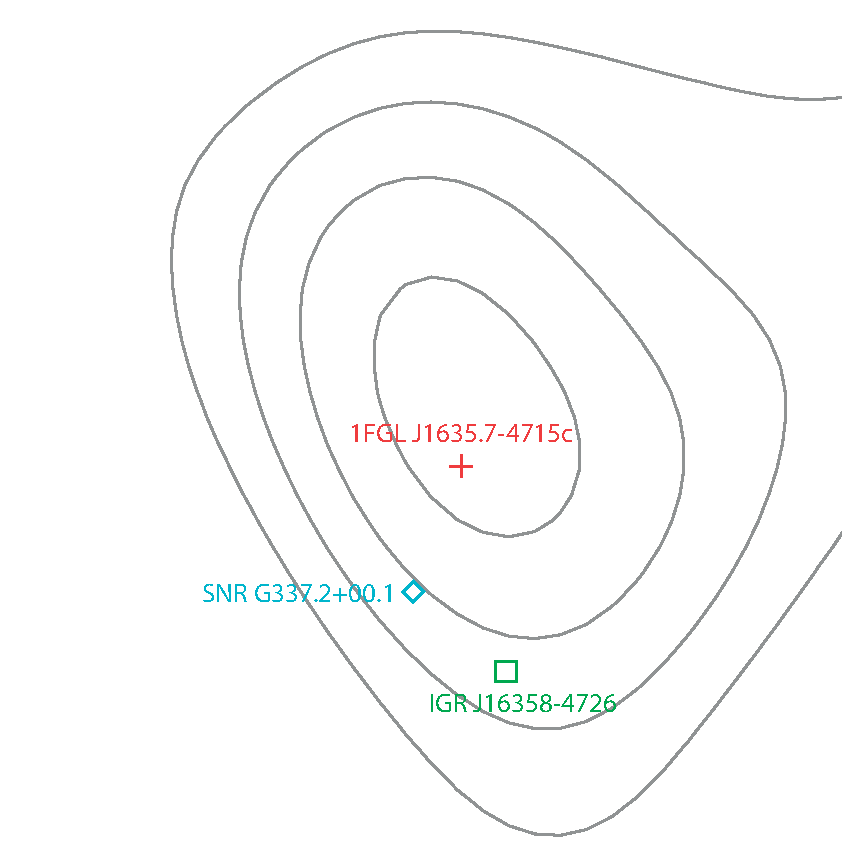
\includegraphics[width = \columnwidth]{figures/hess34}}
  \caption{Contour plot of HESS J1634-472 and surrounding objects of interest. Wolf-Rayet stars are shown as red crosses, supernova remnants as blue diamonds, and pulsars as green squares}
  \label{fig:hess34}
\end{figure}

\paragraph{}
There's an intersting pulsar IGR J16358-4726, but the two WR*s near that pulsar are pretty awful.

\subsubsection{IGR J16358-4726}
\paragraph{}
Also known as [KRL2007b] 194, this object is well within the bounds of HESS J1634-472, as depicted in Figure~\ref{fig:hess34}. Occasionally observed since the late nineties, it was not until 2003, when the object was serendipitously detected by \textcite{Patel:2004} at the Chandra X-Ray Observatory, that it was classified as an X-ray transient owing to its nature of only being visible for brief periods of time, and showing significant fluctuations in its energy output. \textcite{Nespoli:2010} proposed that IGR J16358-4726 is actually one of only a handful of symbiotic X-ray binaries (SyXBs), a new subclass of low-mass X-ray binary systems. SyXBs are believed to feature a compact object (i.e., white dwarf, neutron star, or black hole) orbiting and accreting matter from an M-type red giant star.

The kinematic analysis of the gas bubble around this pulsar outlined earlier provided figures of \unit{9.34\e{42 \mathrm{~to~} 44}}{\joule} for the near solution of \unit{4.18}{\kilo\parsec} and \unit{1.78\e{44 \mathrm{~to~} 46}}{\joule} for the far solution of \unit{11.2}{\kilo\parsec}. As mentioned, supernovae typically emit around \unit{10^{44}}{\joule} \parencite{Khokhlov:1993}, so this result may actually make it far more likely that the near solution is correct, since values less than \unit{10^{44}} are much more likely than those above.

\subsubsection{Wolf-Rayet stars}
\paragraph{}
2MASS J16345746-4704129 is 3.71 kpc

\subsection{HESS J1640-465}

\begin{figure}[H]
  \centering
  \frame{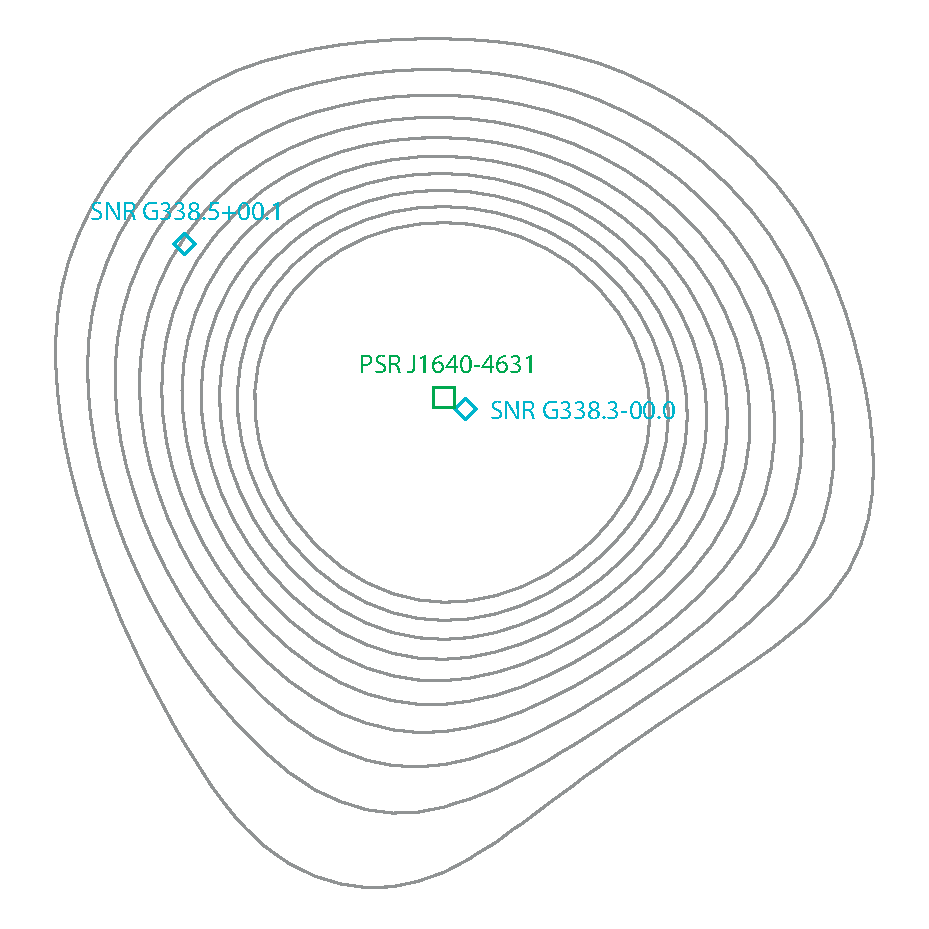
\includegraphics[width = \columnwidth]{figures/hess40}}
  \caption{Contour plot of HESS J1640-465 and surrounding objects of interest. Supernova remnants are shown as blue diamonds and pulsars as green squares}
  \label{fig:hess40}
\end{figure}

\paragraph{}
HESS J1640-465, at an estimated distance of \(12\) to \unit{13.5}{\kilo\parsec} is the most luminous TeV source in the galaxy \parencite{Gotthelf:2014}, with a flux greater than \unit{200}{\giga\electronvolt} of \unit{20.9\pm2.2\e{-12}}{\photon\usk\centi\metre\rpsquared\usk\reciprocal\second} \parencite{Aharonian:2006}.

\subsubsection{PSR J1640-4631}
\paragraph{}
HESS J1640-465 has a SNR counterpart G338.3-0.0, where 2007 keV X-ray observations found an object near the centre of G338.3-0.0. These observations were theorised to be caused by synchrotron emission from a PWN \parencite{Funk:2007}. \textcite{Funk:2007} suggest that if a corresponding pulsar could be detected then gamma rays would be emitted by inverse Compton scattering in the associated PWN. In 2014 new observations with the new NuSTAR X-ray telescope discovered the pulsar PSR J1640-4631 with period 206 ms within G338.3-0.0 \parencite{Gotthelf:2014}. \textcite{Gotthelf:2014} explains that it is not possible to distinguish between any emission that occurs in the SNR shell and the PWN. \textcite{Gotthelf:2014} mentions that multiple mechanisms are likely to contribute to the extreme gamma ray luminosity of HESS J1640-465.

\section{Conclusions} % finish properly
\paragraph{}
TO DO

Bitch, we concluding now, making the statements that make a conclusion possible to be made with the words and the mouth. Bitch, we're flawless give us good grades.
\end{multicols}

\printbibliography[heading = bibintoc] % Include bibliography entry in ToC

\newpage

\appendix

\section{Derivation of galactic doppler shift}
\label{app:doppler}
\paragraph{}
Here we derive the equation found in Section~\ref{sec:gal-rot}. Looking at Fig.~\ref{fig:doppler}, we can (probably not) see the setup we're going to be dealing with here. In order to derive the velocity along the line of sight in the galactic plane, it is necessary to first consider the velocity field of the galactic plane. With coordinates centred on the GC, the velocity field can be expressed as
\begin{equation}
  \label{eq:vel-field}
  \mathbf{v}(x,y)=v(R)\cdot\!\left(\frac{y}{R},-\frac{x}{R}\right)\;,
\end{equation}
where \(x\), \(y\) are the Cartesian coordinates of point P, and \(R\) is the radial distance from point P to the GC, which by Pythagoras fulfils
\begin{equation}
  R^2=x^2+y^2\;.
\end{equation}

\begin{figure}[h]
  \centering
  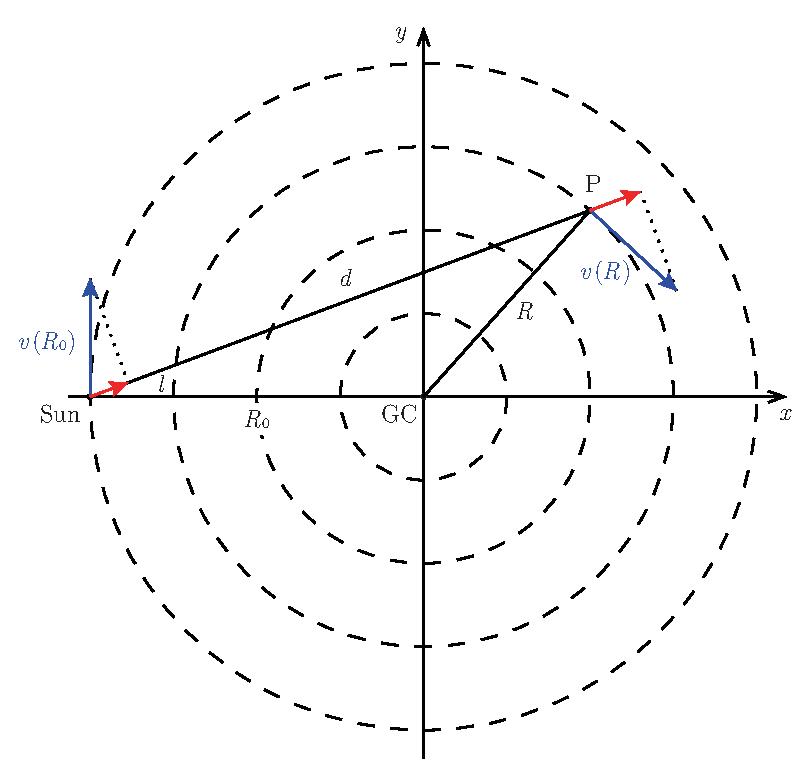
\includegraphics[width=13cm]{figures/doppler-shift}
  \caption{Velocity along line of sight in the galactic plane}
  \label{fig:doppler}
\end{figure}

In Eq.~\eqref{eq:vel-field}, \(v(R)\) is the radial velocity at point P with dependence on \(R\). This velocity field has galactic radial velocities pointing counter clockwise, which is what would be expected of a model for the Milky Way. In order to compute the component of velocities along the line of sight, it is worth considering first the dot product of the velocity field with the direction vector in the direction of the line of sight, \(\mathbf{\hat{d}}\):
\begin{align}
  \mathbf{v}(x,y)\cdot\mathbf{\hat{d}}&=v(R)\left[\left(\frac{y}{R},-\frac{x}{R}\right)\!\cdot(\cos{l},\sin{l})\right] \\
  &=v(R)\left(\frac{y\cos{l}-x\sin{l}}{R}\right) \\
  &=v(R)\left(\frac{y\cos{l}-x\sin{l}}{\sqrt{x^2+y^2}}\right)\;.
  \label{eq:vel-dot}
\end{align}
This expression gives the component of velocity in the \(\mathbf{\hat{d}}\) direction for any \((x,y)\). In order for this expression to be of any use in calculating the Doppler shift from the Mopra data, the coordinates need to be constained to the line of sight. The equation for the line of sight is given in vector form as:
\begin{equation}
  \lambda(d,l)=(d\cos{l}-R_0,d\sin{l})\;\,.
\end{equation}
Substituting the \(x\)- and \(y\)-coordinates from this expression in to Eq.~\eqref{eq:vel-dot} and expanding gives
\begin{equation}
  v_{los}(d)=\frac{v(R)R_0\sin{l}}{\sqrt{d^2-2R_0d\cos{l}+R_0^2}}\;\,.
\end{equation}
This expression only yields the absolute motion in the galaxy, and it is easy to see that for \(d=0\), \(v(0)=v(R)\sin{l}\) -- the sun's component of velocity along the line of sight. Subtracting this value gives us the equation used in the analysis of Mopra data:
\begin{equation}
  v_{los}(d)=\frac{v(R)R_0\sin{l}}{\sqrt{d^2-2R_0d\cos{l}+R_0^2}}-v(R_0)\sin{l}\;\,.
\end{equation}
In order to compute distances for a given velocity, the above equation can be rearranged to give
\begin{equation}
  d=R_0\left(\cos{l}\pm|\sin{l}|\sqrt{v_{rel}^2-1}\right)\;,
  \label{eq:d}
\end{equation}
where \(v_{rel}\) is defined to be `relative' velocity,
\begin{equation}
  v_{rel}\equiv\frac{v(R)}{v_{los}+v(R_0)\sin{l}}\;\,.
\end{equation}

\section{Derivation of kinetic energy of expanding bubble}
\label{app:kinetic}
\paragraph{}
Here we derive the equation found in Section~\ref{sec:kinetic}. We begin with the familiar nonrelativistic equation for kinetic energy,
\begin{equation}
  \mathrm{KE} = \frac{1}{2} m v ^ 2 \, ,
\end{equation}
where \(m\) is the mass of the material displaced by the bubble (typically somewhat of an estimate) and \(v\) is the speed at which the bubble is expanding, i.e., the average speed of the gas in the reference frame of the object presumed to be at the centre. Mass \(m\) is given by mass density \(\rho\) multiplied by volume \(V\), and \(v\) can be found by halving the difference in speeds \(v_1\) and \(v_2\) of the front and back of the bubble:
\begin{equation}
  \mathrm{KE} = \frac{1}{2} \rho V { \left( \frac{\lvert v_1 - v_2 \rvert}{2} \right) }^2 \, .
\end{equation}
The volume \(V\) of the bubble is given by its radius, hence,
\begin{equation}
  \mathrm{KE} = \frac{1}{8} \rho \left( \frac{4}{3}\pi r^3 \right) {(v_1 - v_2)}^2
\end{equation} \begin{equation}
  \mathrm{KE} = \frac{1}{6} \pi \rho r^3 {(v_1 - v_2)}^2  \, .
\end{equation}
To find the radius of the bubble, we first determine the image slice which is halfway between the front and back slices of the bubble, ideally giving us a view of the bubble's cross section at the centre. Using Eq.~\ref{eq:d} outlined at the end of Appendix~\ref{app:doppler}, we can find the distance \(d\) to this slice. Now, consider a circle of radius \(d\) with its origin centred on the Solar System. This circle has a circumference of \(l = 2 \pi d\), and passes through all objects which are located a distance \(d\) away from us, including the middle of our chosen bubble. If we measure the angular width \(\Delta l\) of the bubble in degrees, then by a simple ratio the bubble has diameter \(\frac{\Delta l}{360}l\). Note this is diameter and not radius, so to get \(r\) we then halve this result. Thus,
\begin{equation}
  \mathrm{KE} = \frac{1}{6} \pi \rho {\left( \frac{1}{2} \frac{\Delta l}{360} 2 \pi d \right)}^3 {(v_1 - v_2)}^2  \, ,
\end{equation}
and we rearrange to get our final result:
\begin{equation}
  \mathrm{KE} = \frac{\pi ^ 4}{6} {\left( \frac{\Delta l}{360} \right)}^3 \rho d^3 {(v_1 - v_2)}^2 \, .
\end{equation}

\newpage

\section{Observation table for Mopra \elem{12}{C}O and \elem{13}{C}O data cubes} \label{app:obs-table}
\begin{table}[H]
\centering
\caption{Observations made using Mopra \elem{12}{C}O and \elem{13}{C}O data cubes}
\vspace{1em}
\begin{tabular*}{\textwidth}{@{\extracolsep{\fill} } l *{5}{c} p{5cm}}
\hline \hline
System         & \(l\) (J2000) & \(b\) (J2000) & \(z_1\) \((\metre\usk\reciprocal\second)\) & \(z_2\) \((\metre\usk\reciprocal\second)\) & \elem{x}{C}O & Notes \\
\hline
Pulsar          & 336.91 &  0.055  & -120753  & -117072  & 12 &
                Tenuous cloud hovering around PSR J1635-4735, but no obvious bubble \\
Pulsar          & 337.14 &  0.020  & -114882  & -117072  & 12/13 &
                Sharp gradient, possible SNR interaction? [KRL2007b] 194, SNR G337.2+00.1, 2MASS J16355116-4719515 \\
Star            & 336.43 & -0.262  & -92488.2 & -85430.7 & 13 &
                Strong cloud correlation in 13CO to masers below galactic plane \\
Pulsar/Star     & 336.36 & -0.137  & -83047.6 & -78648.2 & 13 &
                Activity in 13CO focused around masers and another A-type star HD 330913. Also, perhaps related to pulsar PSR J1633-4805 \\
X-ray           & 336.88 &  0.120  & -82811.4 & -75713.9 & 12 &
                Cloud hovering below x-ray emission \\
Maser/Pulsar    & 336.84 &  0.014  & -82548.6 & -68353.5 & 12 &
                Sharp gradient around PSR J1635-4735 \\
Pulsar          & 337.10 & -0.088  & -78605.5 & -74662.4 & 12 &
                Nebulous cloud around [KRL2007b] 194, could be other side of jet? PSR J1637-4721 \\
SNR/Pulsar      & 337.21 &  0.055  & -75012.9 &  -63096  & 12 &
                Steep gradient around SNR G337.2+00.1 Combinations from [KRL2007b] 194, 2MASS J16355116-4719515, 2MASS J16354434-4719422 ? \\
WR*             & 336.30 &  0.200  & -49868.3 & -44918.9 & 13 &
                Active 13CO cloud presence with correlation to band of WR stars ? \\
WR*             & 336.55 &  0.160  & -42352.6 & -40519.5 & 13 &
                13CO activity near WR stars {2MASS J16324979-4744314} {2MASS J16324808-4744493} \\
WR*/Pulsar      & 337.20 &  0.400  & -46660.2 &  -40336  & 13 &
                Possible bubble and jets, could be from WR star {2MASS J16345746-4704129}. Nearby pulsar {PSR J1637-4642} may have single jet coincidentally extending until -39419.4 \\
SNR/Pulsar      & 338.48 &  0.020  &  -43994  & -36458.3 & 12/13 &
                Massive gradient near B9IV star, HD 328664. In 13CO there is a strong suggestion of a bubble relating the activity to SNR G338.5+00.1! Suspect also to be the cause of surrounding masers \\
\hline
\end{tabular*}
\label{tab:mopra-obs}
\end{table}
\vspace{-1em}
{\footnotesize The \(z_1\) and \(z_2\) columns show the doppler shifts of the slices at the beginning and end of each observation in the data cube. The \elem{x}{C}O column shows observations made in either \elem{12}{C}O, \elem{13}{C}O, or both.}

\end{document}